\documentclass[a4paper,12pt]{article}
\usepackage{filecontents}
\usepackage{graphicx}
\usepackage{epstopdf}
\begin{filecontents*}{refs.bib}
@BOOK
{Boulund,
    AUTHOR    = "Fredrik Boulund and Anna Johnning and Mariana Buongermino Pereira and DG Joakim Larsson and Erik Kristiansson",
    TITLE     = "{A novel method to discover fluoroquinolone antibiotic resistance (qnr) genes in fragmented nucleotide sequences}",
    PUBLISHER = "BMC Genomics",
    YEAR      = 2012
}
\end{filecontents*}
\usepackage[style=authoryear-ibid,backend=biber]{biblatex}
\addbibresource{refs.bib}

\title {Report on project in MVE405!}
\date {Aug 21, 2013}

\begin{document}

\maketitle

\section{Abstract}
This report documents the outcome of a project in the Chalmers course MVE405 - Individual project in mathematics and mathematical statistics.

\subsection{Background}
\textcite{Boulund} published a method with an accompanying Python-based tool for identifying fluoroquinolone antibiotic resistance (qnr) genes using Hidden Markov Models (HMM) and gene clustering techniques in metagenomic datasets. While giving satisfactory results for that particular case, it was difficult both to use the pipeline for more complex models, other types of data and huge datasets. This report documents a project that aims to generalize, modularize and optimize the pipeline to both expand its use cases to identify, for example, beta-lactamese enzymes, while enabling it to work on huge sets of short, fragmented reads on the scale of tens of terabases (TB).

\subsection{Results}
While retaining the original method and statistical power of the original pipeline, the new toolset - named SofT - enables a fast and easy way to combine substeps in hierarchical and parallell order to use several Hidden Markov Models. This report will also show that new functionality enables analysis of either nucleotide or amino acid representation of sequences in subsequent steps, which provides both flexibility and confidence when fragments are later assembled as nucleotides after an initial filtering an analysis of their possible translations as proteins. Finally, datasets of arbitrary size can be used as input and we will explore the feasability with regards to memory, storage and computational time. The main part of the project has been revolving around the technical design and implementation of the new toolchain, and this will be reflected in the report.

\section{Results}
\subsection{Overview}
SofT is developed for Python 2.6, but should run fine under 2.7 as well. For details on installation and dependencies, refer to the online documentation.

The main purpose of SofT is to find potential known and putative genes in a set of metagenomic samples consisting of short reads. This is done first by filtering and then by attempting to assemble the remaning fragments. Being a pipeline, running SofT is a process consisting of several distinct steps. The modules definig the behavior of these steps are called \emph{sieves}. Each sieve will take an input file with sequences in FASTA or FASTQ format to process, optionally with two reference databases - one for nucleotide sequences and one for protein translations - generated by any previous sieves in the current execution. After processing, it in its turn generates a new output file of similar format with reference databases. Generally, an output FASTA file is used as input data in the next sieve while the databases are used as backreference to quickly retrieve either representation of the sequence from an id. Databases also store metadata generated during a run, such as scores for how well the sequences match the gene prediction model. If a pipeline is to be rerun on a dataset, it can easily be started from any position in the process to avoid unnecessary recalculation of already derived results. For example, the readfasta sieve rarely has to be run more than once for any dataset and the resulting files can be reused with other models.

Input is supplied as nucleotide sequences in FASTA or FASTQ format, in clear-text or gzipped. The treatment of the input file is determined by the filename ending.

\subsection{qnr sieve example}
Below, we will briefly use the qnr gene identification case used in Boulund's original pipeline as an example to illustrate the flow and structure of SofT and the presupplied sieves. See figure~\ref{fig:qnrflow} for an illustration.

\begin{figure}[h]
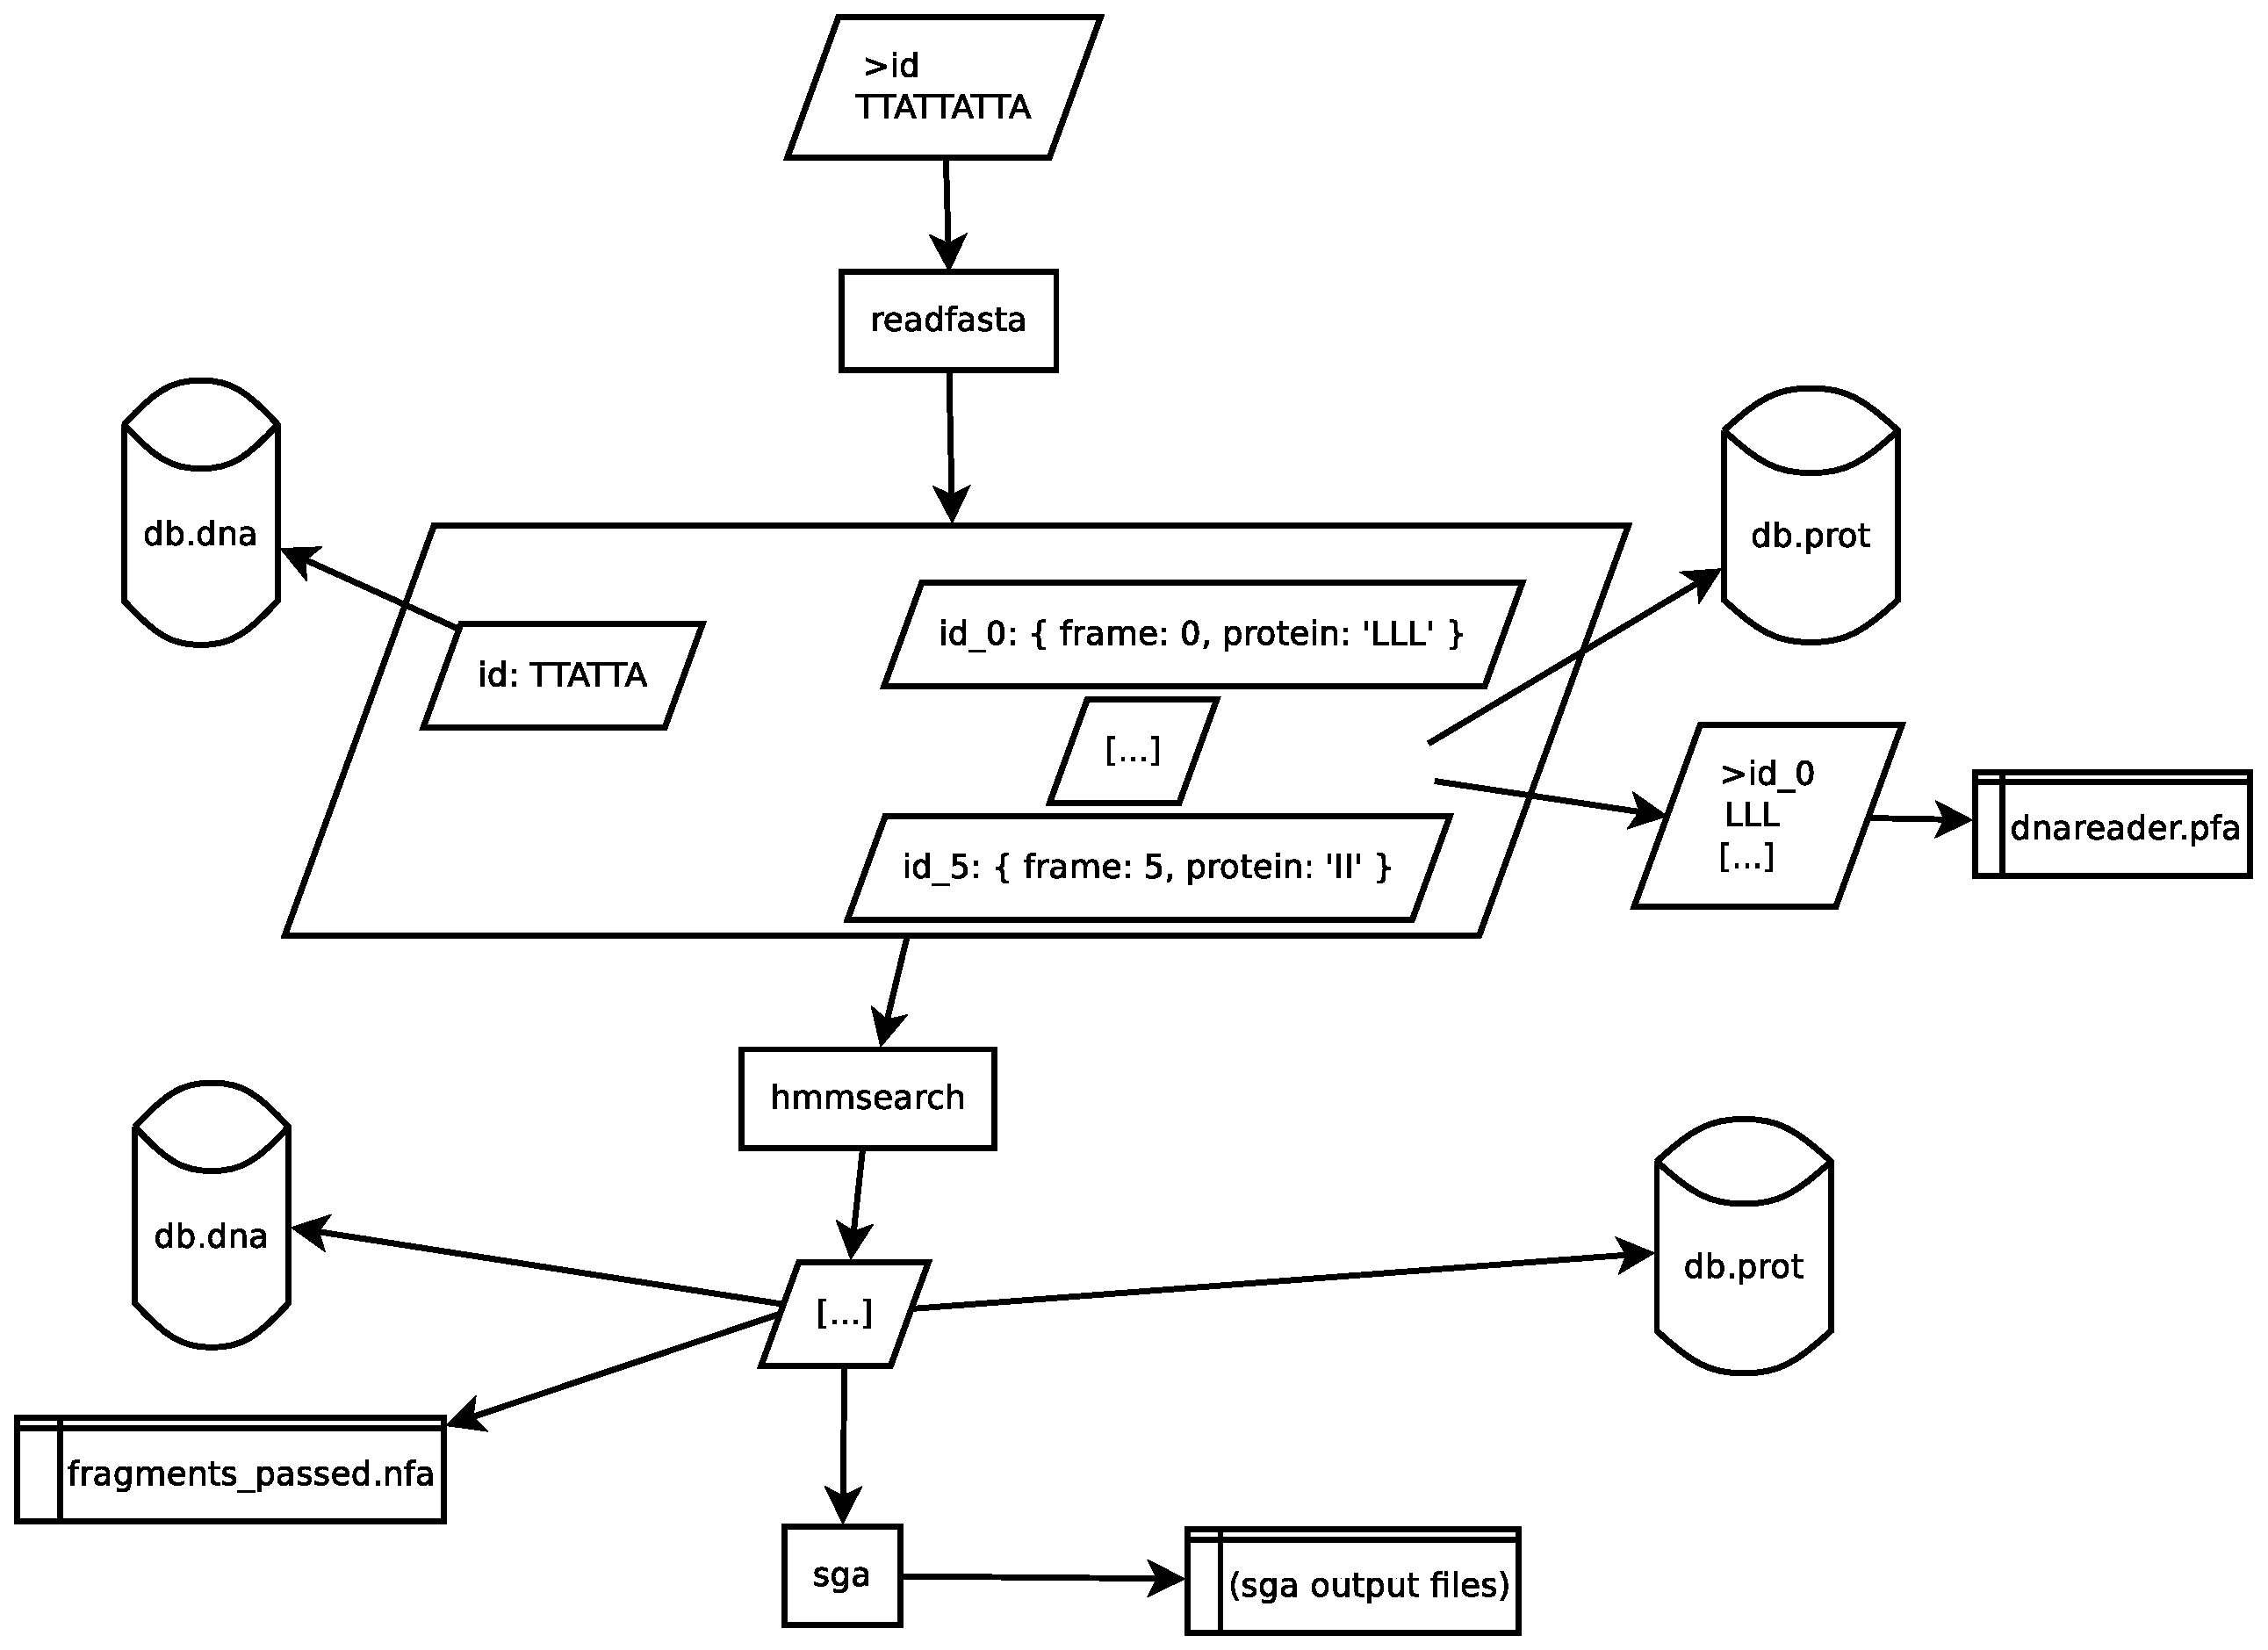
\includegraphics[width=\textwidth, keepaspectratio=true]{flow}
\caption{Flow for qnr sieve sample. The structure of the output data of all sieves are the same. For the sake of brevity, only the first is shown in detail.}
\label{fig:qnrflow}
\end{figure}

\subsubsection{readfasta}
The first step in any pipeline will usually be a preprocessing step performed by the \emph{readfasta} sieve. It simply translates the nucleotide sequences in the input files to amino acids in all six reading frames and outputs the result to database files and an output text file. This is generally the most time-consuming step.

\subsubsection{hmmsearch}
The hmmsearch sieve takes a FASTA file with protein sequences and performs a HMMER hmmsearch against a predefined model file. Only sequences whose domain score passes a predetermined classification function will be outputted. The default classification function is the one derived from the results in \cite{Boulund}. In the qnr case, only the matching domain is written to the output file and used for assembly.

\subsubsection{sga}
The output sequences from hmmsearch are considered as potential fragments from qnr genes. As input is usually from metagenomic samples sequenced from so-called Next-Generation Sequencing technologies such as Illumina, an attempt to assemble them into full-length genes is made. In this case, the String Graph Assembler (SGA) package is used. Since SGA doesn't keep a reference to the fragments that form a contig, this information is lost. Furthermore, the non-zero error tolerance rate (default 0.02) makes it non-trivial to derive from the databases. As a consequence, the current implementation of SGA does not put anything in its output databases but only generates output files with the resulting contigs. This could, in the future, be resolved by using an aligner such as MAFFT.

\subsection{beta-lactamase example}
The beta-lactamase sample functions as the qnr one, with a notable difference. The different classes of qnr genes can be classified using a single hmmer model. The structure of beta-lactamase genes makes this more difficult for them. To get satisfactory results, a hierarchical model is used: An overall model used to classify as potential qnr or not, with a subsequent model for each of the serine-based subclasses. This suggests a hierarchical model, illustrated in figure~\ref{fig:blflow}.
For any input file, three output files will be generated. The three processes could be run in parallell, but this is not done in the current implementation; both HMMER and SGA can be adjusted to run their individual processes across several threads either way, so it should not provide much of a performance improvement. Worth to note is that the first general hmmsearch run outputs the matching sequences in their entirety while the submodel runs trim the output down to only the matching domain just as in the qnr case above.


\begin{figure}[h]
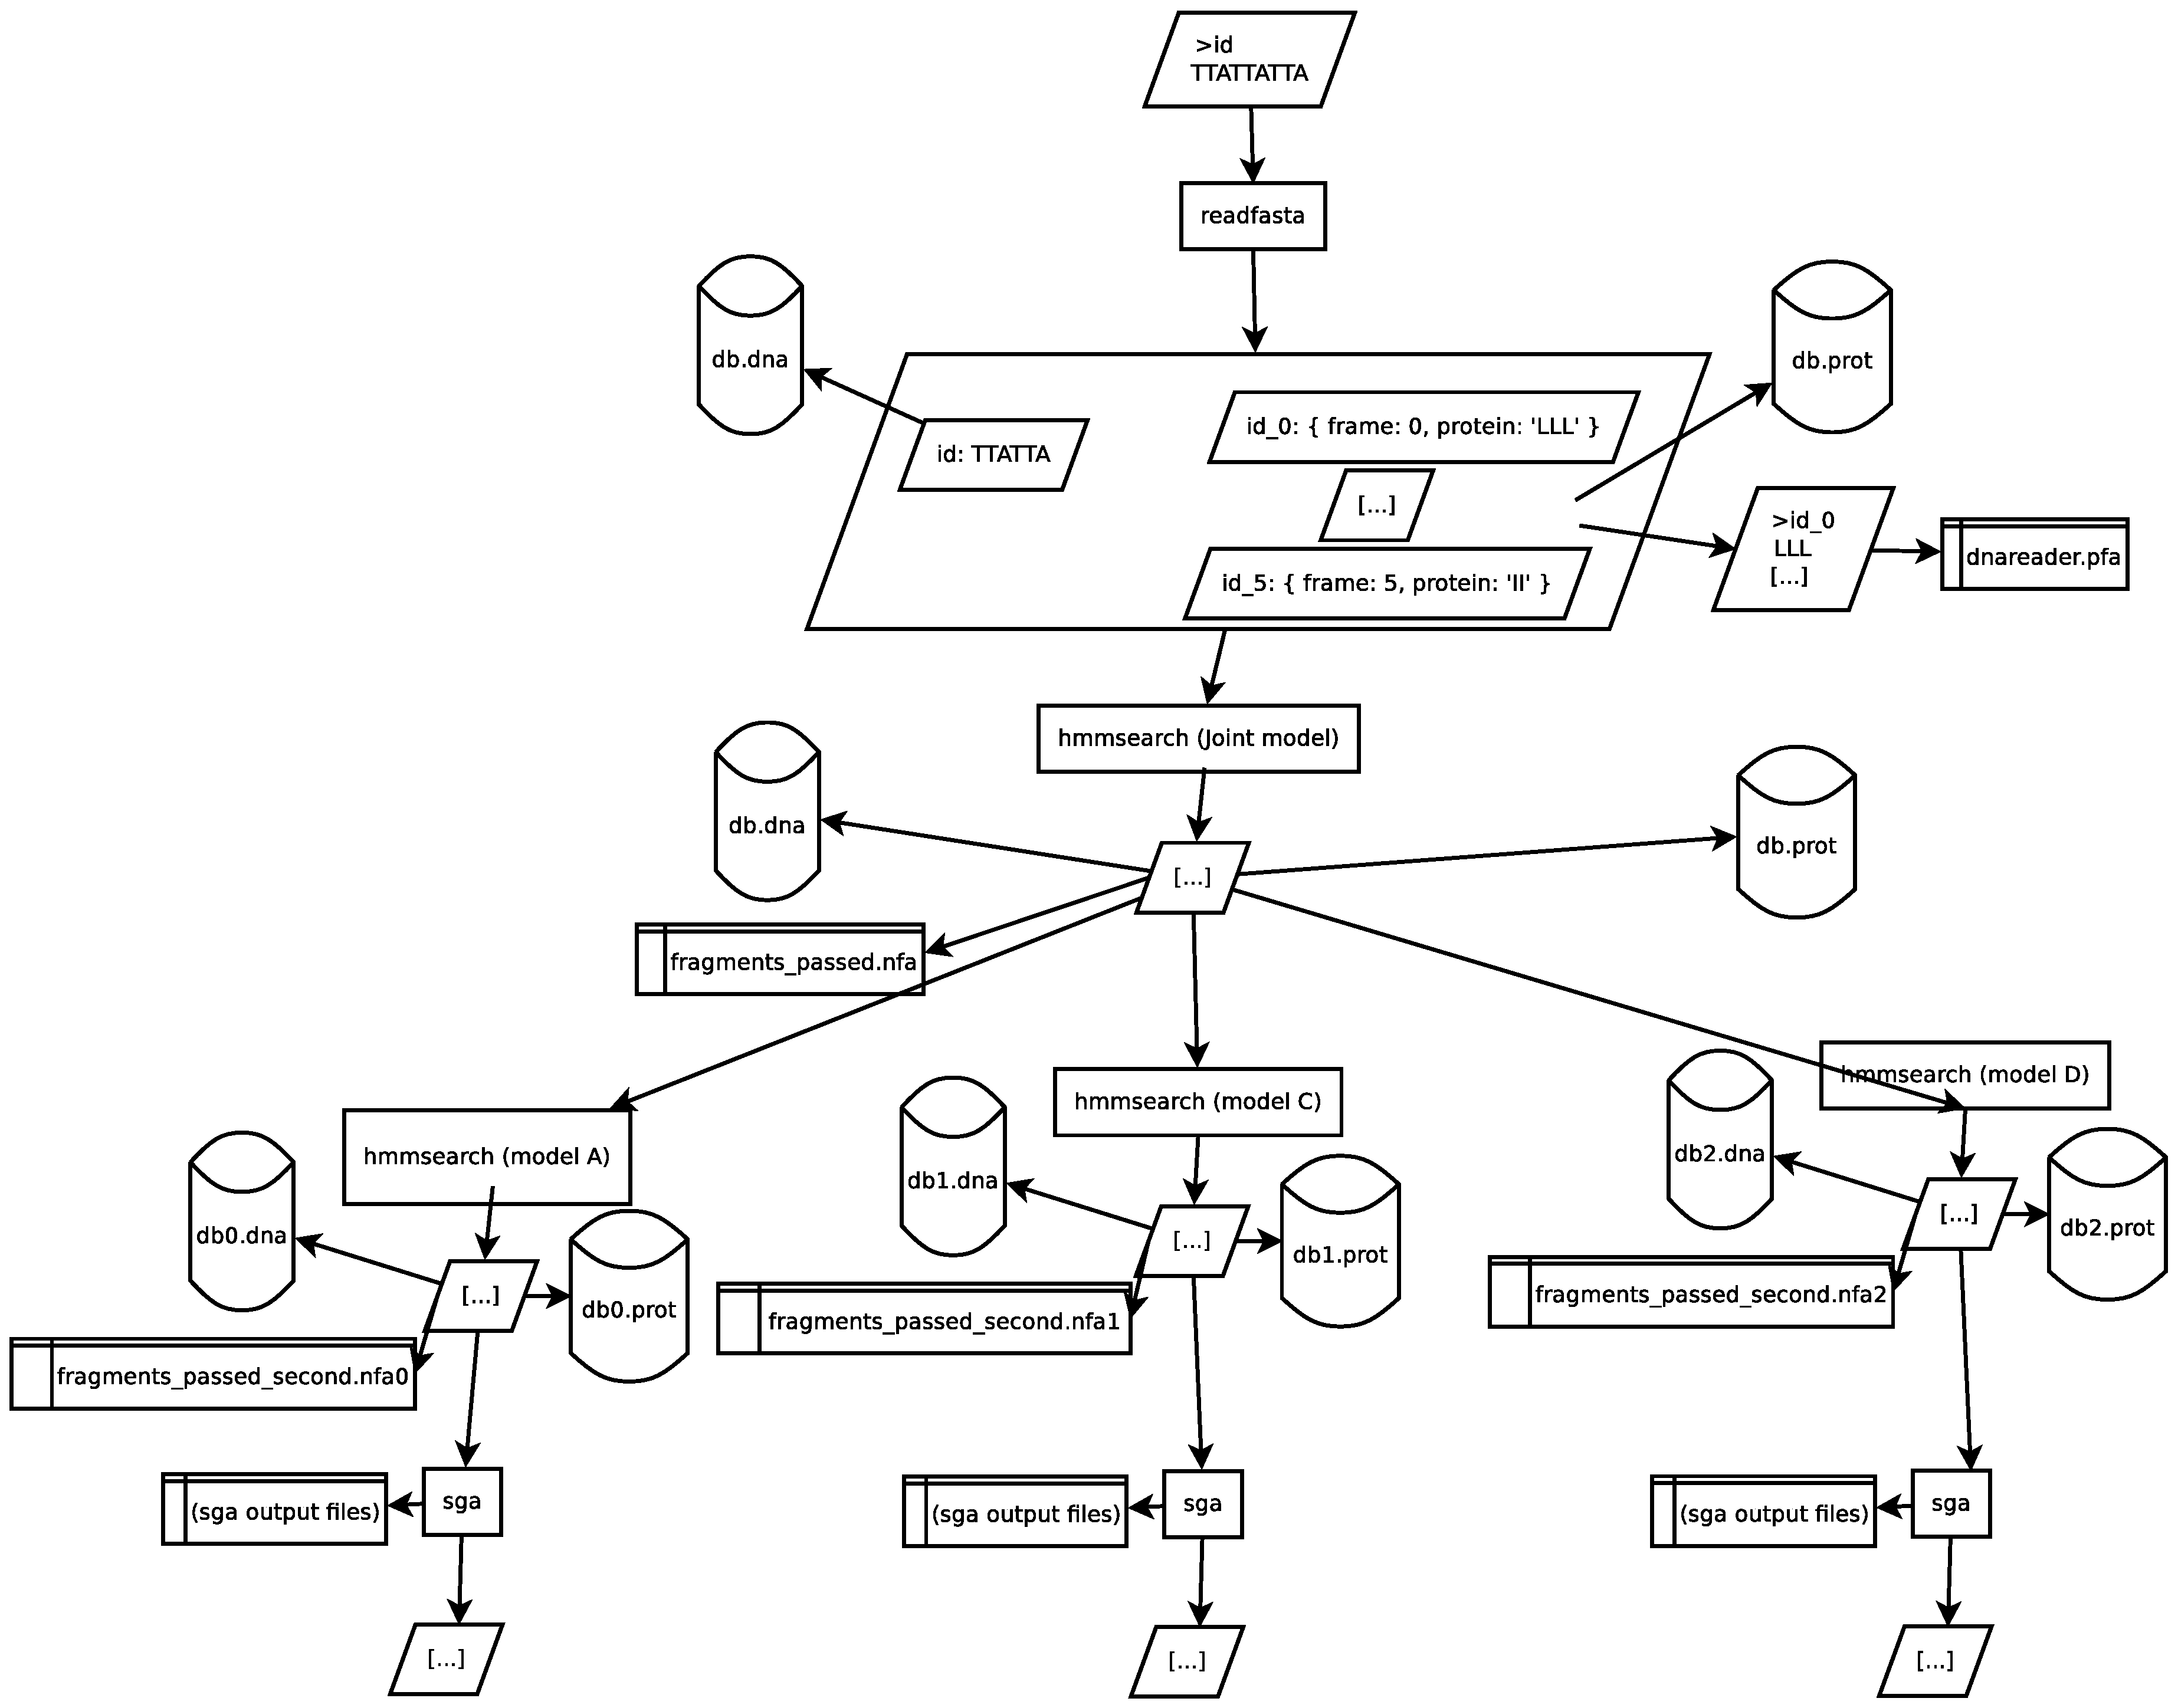
\includegraphics[width=\textwidth, keepaspectratio=true]{blflow}
\caption{The hierarchical flow used in the betalactamase sample. Each serine subclass creates an individual fork of the sieve for the rest of the run.}
\label{fig:blflow}
\end{figure}

\subsection{Selecting parameters for the sieves}

To get satisfactory results, it is of vital importants to give good parameters to hmmsearch and SGA. The first key here is, as always, to know your data. To aid in the process of evaluating parameters, a wrapping sieve called multi-runner is included. We will show how this sieve was used to choose the supplied default values for the sga sieve.

\subsubsection{The multirunner}
The supplied \emph{multirunner} sieve has only two mandatory parameters: another sieve, and a set of parameters, each with a list of parameter values. When executed, it runs the sieve once for every possible combination of parameter values, storing the results in separate files. This automates the task of evaluating the effect of different parameter values.

\subsubsection{Parameters for SGA}
SGA (String Graph Assembler) is a complex pipeline in itself, with several parameters to tweak that will heavily influence the result of an assembly. It is thus important to pick the variables carefully in order to get sane results. In order to select the default values for the SGA sieve, an evaluation set was created by taking seven known qnr genes and randomly slicing and mutating them, creating a file with 100 basepairs long sequences. The script that was used to do this is included in scripts/fb\_fragments\_from\_fasta.py, with a random mutation rate of 1\%.

The evaluated parameters and their values tested:
\begin{itemize}
\item
error\_rate: [0.01, 0.02, 0.03],
\item
min\_assembly\_overlap: [0, 5, 10, 15, 20, 25, 30],
\item
min\_merge\_overlap: [5, 10, 15, 20, 25, 30],
\item
resolve\_small: [0, 5, 10, 500]
\end{itemize}

Running the multirunner sieve with these paramaters initiated an SGA sieve run with each of all the possible combinations of these values. Output sets were then sorted based on contig count, average contig length and length of longest contig. They were then manually evaluated. Balanced results seemed to be achieved with the following values:
\begin{itemize}
\item
error\_rate: 0.02
\item
min\_assembly\_overlap: 20
\item
min\_merge\_overlap: 20
\item
resolve\_small: 5
\end{itemize}
This gave 54 contigs with an average length of 84 and a longest contig length of 592. This seems to suggest that further scaffolding or alignment might be needed to get really meaningful results. Since the scaffolding part of SGA requires paired-end or mate pair reads and the framework is designed for a use case with more general data in mind, this option has been discarded for the moment. If this functionality is desired, the SGA sieve can easily be modified accordingly as long as the pairing information is saved in the reference databases.

\subsection{Performance}
The pipeline has been benchmarked on a shared RedHat Linux environment with 16 GB RAM, 4 core 64 bit Intel Xeon X3470 CPU at 2.93 GHz. The operations were performed on an ext4 file system on a RAID spread across 7200 rpm SAS 600 disks with 16MB cache.

Profiling was performed using Python's supplied cProfile module, which generally adds an acceptable overhead REFERENCE. 

Execution time logs for gzip format:
Input: 100 bp Immunina reads

37,168,092 fragments, gzipped = 3,716,809,200 bases $\sim$= 3.7 GB (resulting pfa file: 9.7 GB)

The ext4 file system adds a significant overhead for database writes, so use of another filesystem such as ext3 should significantly improve performance. If large enough SSD disks can be afforded, this could also be considered.

\begin{tabular}{lll}
% (with json) Step 1: Translate DNA to protein and insert both into leveldb database: 3:51:40
Step 1&Translate DNA, insert into database&1:20:39\\
Step 2&hmmsearch (1076 sequences passed)&0:02:14\\
Step 3&SGA&0:00:6
\end{tabular}


$\sim$2.5 GB / h = 0.4 h / GB = 400 h / TB $\sim$= 17 days / TB = 167 days / 10 TB.


 
\subsection{Design choices}
\subsubsection{Translator}
Since input data is in nucleotide format and anlasys is done for amino acids, the input sequences need to be translated before analysis. Boulund's original QNR pipeline used transeq for this purpose. Transeq is stable and has very good performance. However, the output from transeq does not contain any reference to the input sequence. Since the original DNA sequence is used for analysis in later stages and the startup overhead involved in running transeq sequence by sequence was too large to be fast enough, an alternative had to be found. Biopython was evaluated but proved to be too slow. A custom implementation in Python worked better, but even after aggressive optimizations it was still more than ten times slower than transeq and took a considerable fraction of the total running time of the pipeline. The code was ported to Cython, a statically typed superset of Python that compiles to C code with Python bindings. Adding type declarations alone gave significant improvements, and after all the heavy parts of the process had been optimized, it was fast enough so that database and file I/O and serialization were the only significant bottlenecks.

\subsubsection{Serialization}
Sequences and their metadata are stored in dictionaries. In Python, JSON is the fastest serialization option, and the most concise text-based one, which made the choice natural. Unfortunately, there is significant overhead involving type-lookups that slows down the process. Therefore, a string-concatenation-based approach is used for serialization while the bundled json solution is still used for deserialization. Given the low percentage of sequences that make it through in the QNR and beta-lactamase use cases, serialization is performed to a much higher extend than deserialization so the somewhat suboptimal deserialization is still acceptable.

\section{Conclusion}
xxx

\section{Acknowledgements}
I want to thank Erik Kristiansson and Fredrik Boulund at the Mathematical Sciences department at Chalmers for giving me the opportunity to do this project and guiding me along the way. I would also like to thank Mariana Pereira for help with the betalactamase data, and the people at the department for good times.

\printbibliography
\end{document}
